
% ********** Chapter 6 **********
\chapter{SIP Call Component}
\label{sec:SIPCallComponent}

\section{Five layers architecture}

A five layers architecture has to be introduced before illustrate the Third Party Call Controller. The five layers architecture is shown in Figure \ref{fig:FiveLayersArchitecture}. From bottom to top, the five layers are Protocol stack, Abstraction layer, Implementation layer, OOP use-case based API layer and JavaBean for synchronized communication.

\begin{figure}[!hbtp]
\centering
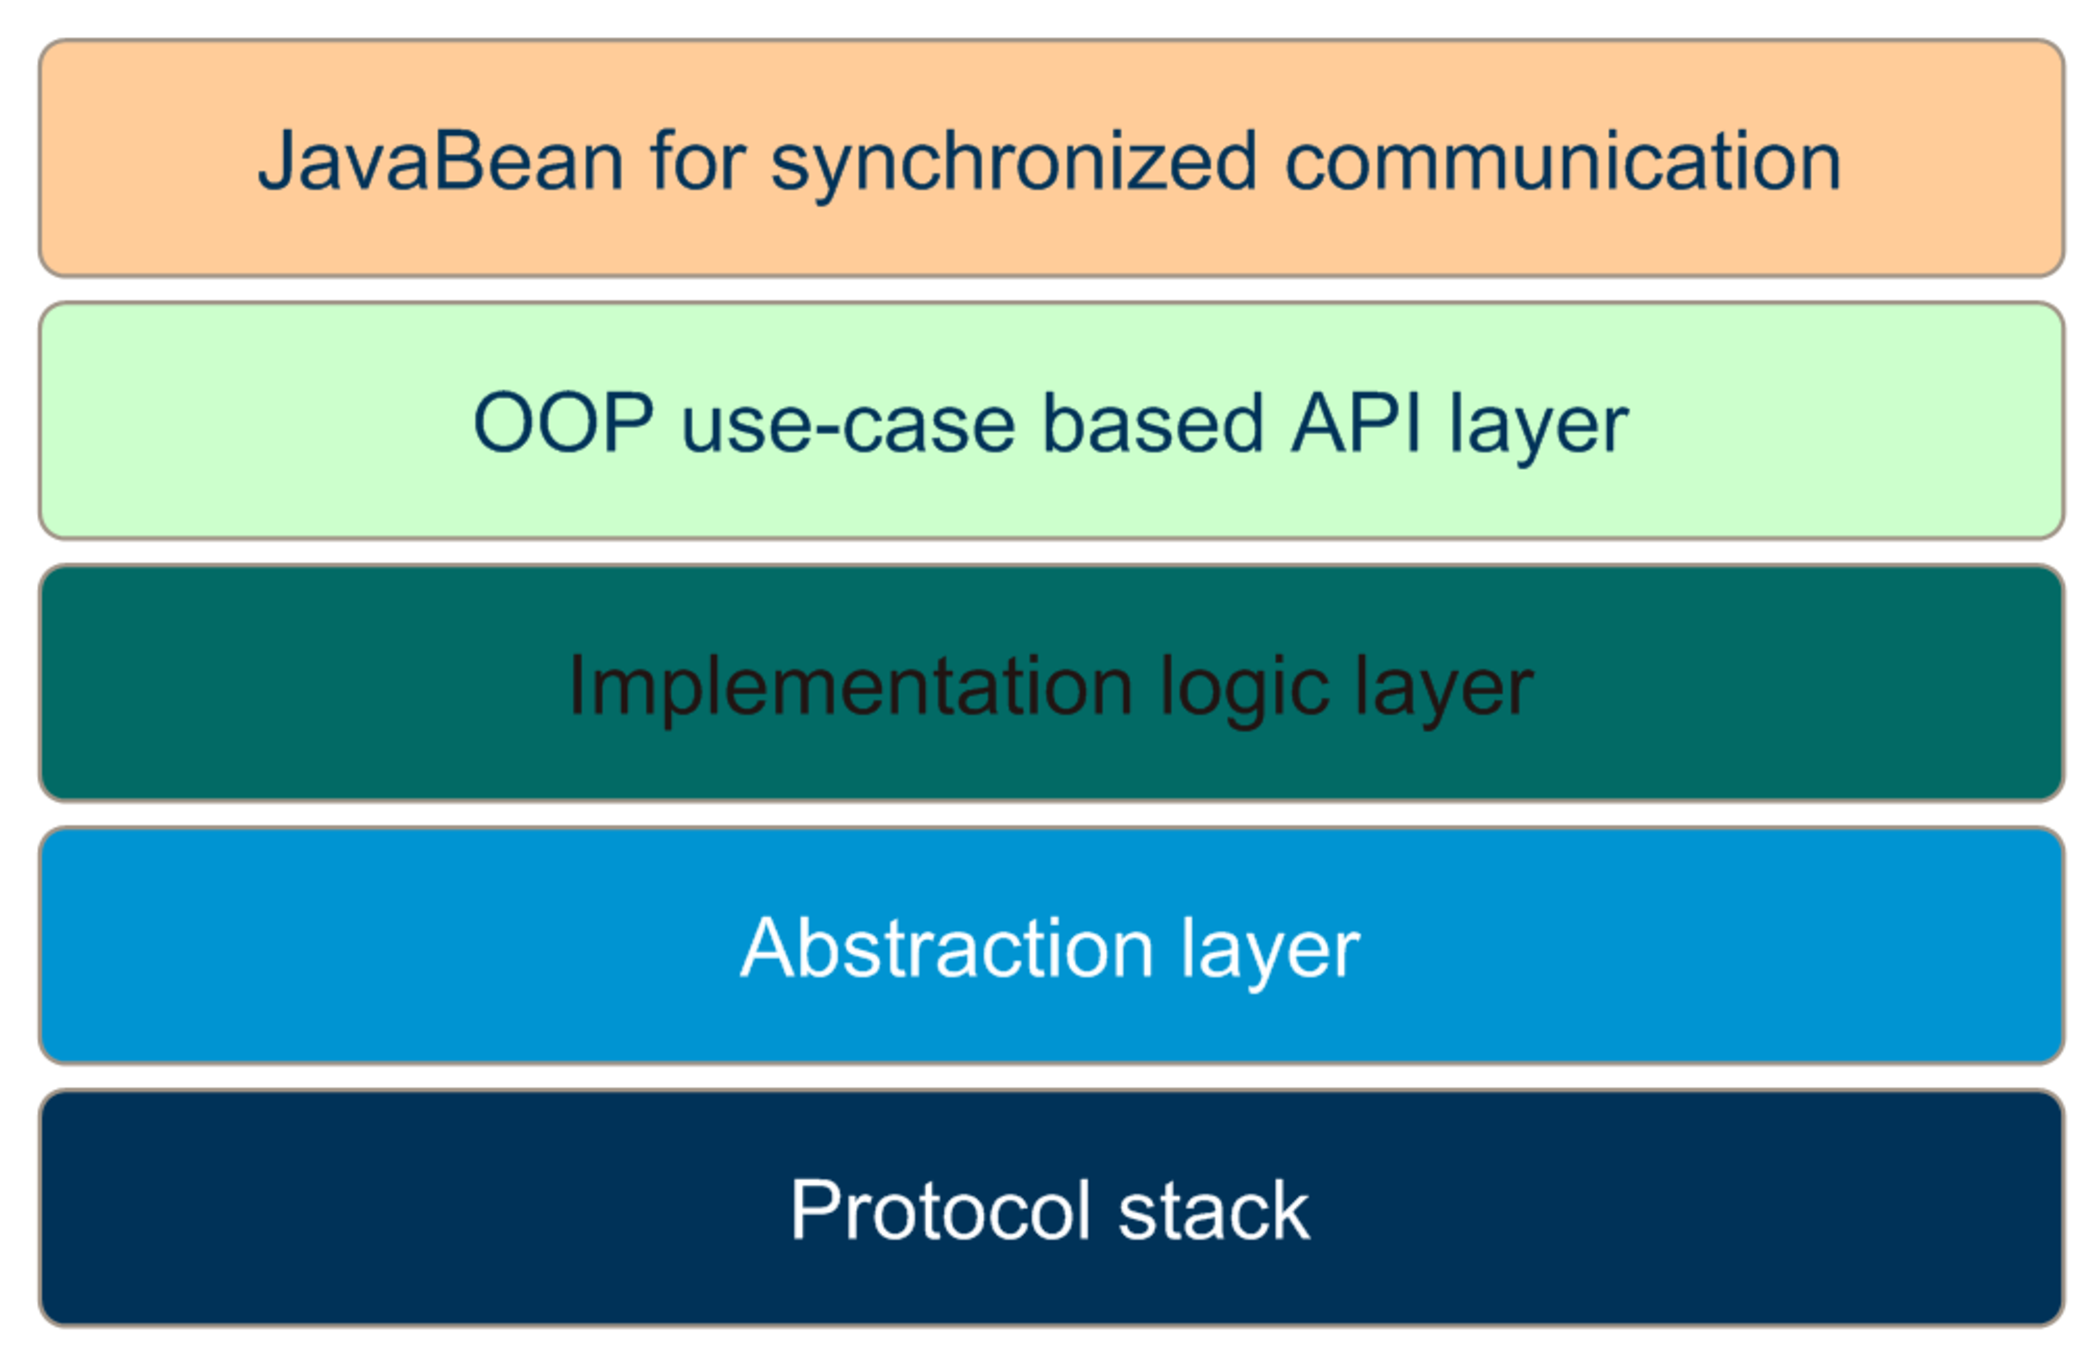
\epsfig{file=chap06/resources/five_layers, width=5.2in}
\caption{Five layers architecture}
\label{fig:FiveLayersArchitecture}
\end{figure}

\subsection{Protocol stack}

The protocol stack is the low level API for the project. There could be several implementations of the protocol stack. 

\subsection{Abstraction layer}

This layer is used for abstracting low level protocol stack. So the project can be easily migrated from one protocol stack to another without modifying the logic layer.

\subsection{Implementation logic layer}

This layer contains the main logic of the project.

\subsection{OOP use-case Based API Layer}

This layer is used for exposing public API for end user. Design Patterns such as Abstract Factory Pattern can be used here, especially for java SE.

\subsection{JavaBean for synchronized communication}

Components in Java are called beans. This layer contains
The JavaBean which special designed for synchronized communication has two pairs of constructor and business logic group. The constructor which has system parameters works with business logic which doesn't have system parameters. The constructor which doesn��t have system parameters works with business logic which has system parameters. In addition, this kind of JavaBean only has method of \texttt{getState()} and no method of \texttt{setState()}.

\section{Architecture of SIP Call Component}

The SIP Call Component is the core of Web Call Example Application. The design architecture of it is shown in Figure \ref{fig:TheArchitectureOfSIPCallComponent}.

\begin{figure}[!hbtp]
\centering
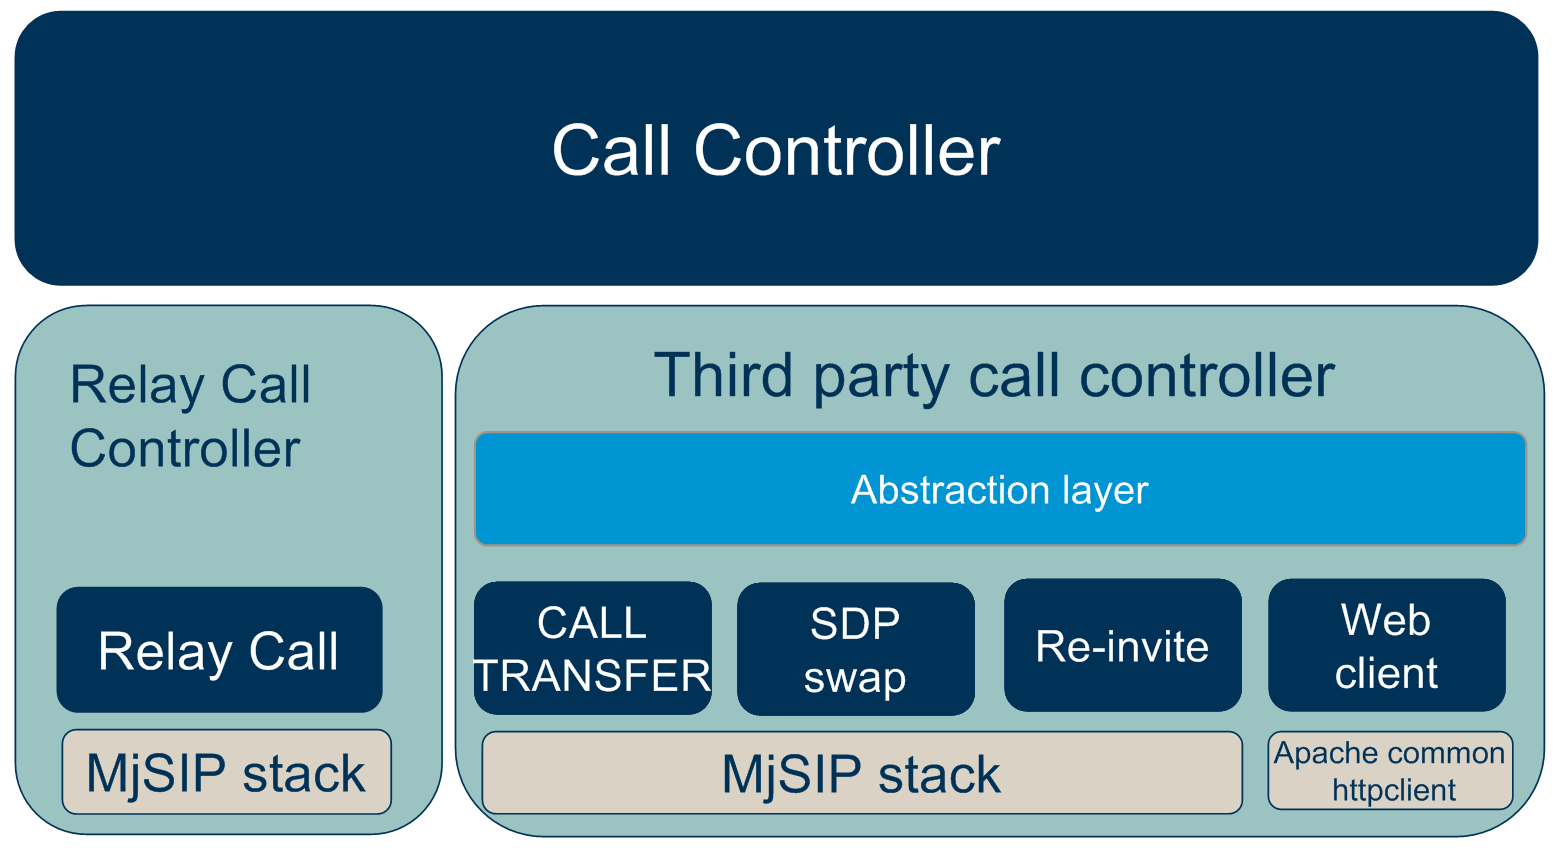
\epsfig{file=chap06/resources/sip_call_component_architecture, width=5.2in}
\caption{The Architecture of SIP Call Component}
\label{fig:TheArchitectureOfSIPCallComponent}
\end{figure}

\textbf{TODO: write something here}

\section{Hierarchy of Call Controller}






% ********** End of chapter **********
